\documentclass[12pt,letterpaper]{article}
\usepackage{graphicx,textcomp}
\usepackage{natbib}
\usepackage{setspace}
\usepackage{fullpage}
\usepackage{color}
\usepackage[reqno]{amsmath}
\usepackage{amsthm}
\usepackage{fancyvrb}
\usepackage{amssymb,enumerate}
\usepackage[all]{xy}
\usepackage{endnotes}
\usepackage{lscape}
\newtheorem{com}{Comment}
\usepackage{float}
\usepackage{hyperref}
\newtheorem{lem} {Lemma}
\newtheorem{prop}{Proposition}
\newtheorem{thm}{Theorem}
\newtheorem{defn}{Definition}
\newtheorem{cor}{Corollary}
\newtheorem{obs}{Observation}
\usepackage[compact]{titlesec}
\usepackage{dcolumn}
\usepackage{tikz}
\usetikzlibrary{arrows}
\usepackage{multirow}
\usepackage{xcolor}
\newcolumntype{.}{D{.}{.}{-1}}
\newcolumntype{d}[1]{D{.}{.}{#1}}
\definecolor{light-gray}{gray}{0.65}
\usepackage{url}
\usepackage{listings}
\usepackage{color}

\definecolor{codegreen}{rgb}{0,0.6,0}
\definecolor{codegray}{rgb}{0.5,0.5,0.5}
\definecolor{codepurple}{rgb}{0.58,0,0.82}
\definecolor{backcolour}{rgb}{0.95,0.95,0.92}

\lstdefinestyle{mystyle}{
	backgroundcolor=\color{backcolour},   
	commentstyle=\color{codegreen},
	keywordstyle=\color{magenta},
	numberstyle=\tiny\color{codegray},
	stringstyle=\color{codepurple},
	basicstyle=\footnotesize,
	breakatwhitespace=false,         
	breaklines=true,                 
	captionpos=b,                    
	keepspaces=true,                 
	numbers=left,                    
	numbersep=5pt,                  
	showspaces=false,                
	showstringspaces=false,
	showtabs=false,                  
	tabsize=2
}
\lstset{style=mystyle}
\newcommand{\Sref}[1]{Section~\ref{#1}}
\newtheorem{hyp}{Hypothesis}

\title{Problem Set 2}
\date{Due: October 14, 2024}
\author{Applied Stats/Quant Methods 1}

\begin{document}
	\maketitle
	\section*{Instructions}
\begin{itemize}
	\item Please show your work! You may lose points by simply writing in the answer. If the problem requires you to execute commands in \texttt{R}, please include the code you used to get your answers. Please also include the \texttt{.R} file that contains your code. If you are not sure if work needs to be shown for a particular problem, please ask.
	\item Your homework should be submitted electronically on GitHub.
	\item This problem set is due before 23:59 on Monday October 14, 2024. No late assignments will be accepted.

\end{itemize}

	
	\vspace{.5cm}
	\section*{Question 1: Political Science}
		\vspace{.25cm}
	The following table was created using the data from a study run in a major Latin American city.\footnote{Fried, Lagunes, and Venkataramani (2010). ``Corruption and Inequality at the Crossroad: A Multimethod Study of Bribery and Discrimination in Latin America. \textit{Latin American Research Review}. 45 (1): 76-97.} As part of the experimental treatment in the study, one employee of the research team was chosen to make illegal left turns across traffic to draw the attention of the police officers on shift. Two employee drivers were upper class, two were lower class drivers, and the identity of the driver was randomly assigned per encounter. The researchers were interested in whether officers were more or less likely to solicit a bribe from drivers depending on their class (officers use phrases like, ``We can solve this the easy way'' to draw a bribe). The table below shows the resulting data.

\newpage
\begin{table}[h!]
	\centering
	\begin{tabular}{l | c c c }
		& Not Stopped & Bribe requested & Stopped/given warning \\
		\\[-1.8ex] 
		\hline \\[-1.8ex]
		Upper class & 14 & 6 & 7 \\
		Lower class & 7 & 7 & 1 \\
		\hline
	\end{tabular}
\end{table}

\begin{enumerate}
	
	\item [(a)]
	Calculate the $\chi^2$ test statistic by hand/manually (even better if you can do "by hand" in \texttt{R}).\\
	
	The $\chi^2$ test statistic quantifies the difference between observed data and what is expected if the null hypothesis is true. The null hypothesis in this case states that the variables are statistically independent ()in this case, that the driver's class does not affect police behavior, or more precisely, does not affect whether bribe is requested).
	
	The formula to find the $\chi^2$ test statistic is:
	
	(number of observances - number that is expected if the samples are fully independent )$^2$/number that is expected if the samples are fully independent
	
	If the null hypothesis (H0) is true we would expected fobserved=fexpected, meaning no significant deviation between observed and expected data. So we are measuring how much the observed data deviates from the expected data under the null hypothesis (samples are independent). 
	
	To do so, I first need to calculate the expected values under H0 (fe). In this context this is the amount of people (not) stopped or bribed in each class if the samples are fully independent, meaning if the class of the driver has no bearing on the behavior of the police.
	
	The formula for this number is:
	
	row total/grand total * column total
	
	Since there are going to be a lot of simple additions in my calculation of the $\chi^2$ test statistic I am going to try to make it less likely I forget part of an equation by already calculating the row/column/grand totals. 
	
	\begin{verbatim}
	> row_1_total<-14+6+7
	> row_2_total<-7+7+1
	> column_1_total<- 14+7
	> column_2_total<- 6+7
	> column_3_total<- 7+1
	> total<- 14+6+7+7+7+1
\end{verbatim}
	
	Then I calculate all the expected values under H0 (samples are independent, fe):
	
			\begin{verbatim}
			up_not<-row_1_total/total*column_1_total
			up_bribe<-row_1_total/total*column_2_total
			up_stop<-row_1_total/total*column_3_total
			low_not<-row_2_total/total*column_1_total
			low_bribe<-row_2_total/total*column_2_total
			low_stop<-row_2_total/total*column_3_total
		\end{verbatim}
		
	I get the following results: 
	\begin{verbatim}
		> up_not
		[1] 13.5
		> up_bribe
		[1] 8.357143
		> up_stop
		[1] 5.142857
		> low_not
		[1] 7.5
		> low_bribe
		[1] 4.642857
		> low_stop
		[1] 2.857143
		\end{verbatim}
	
	With those numbers I can finally calculate my $\chi^2$ test statistic:
	\begin{verbatim}	
	> chi_square<-((14-up_not)^2/up_not)+
	+   ((6-up_bribe)^2/up_bribe)+
	+   ((7-up_stop)^2/up_stop)+
	+   ((7-low_not)^2/low_not)+((7-low_bribe)^2/low_bribe)+
	+   ((1-low_stop)^2/low_stop)
	> chi_square
	[1] 3.791168
		\end{verbatim}
	
	Thus, the $\chi^2$ test statistic equals 3.79. This value measures how much the observed data deviates from the expected data under the null hypothesis (samples are independent).

While this number quantifies the deviation between observed and expected data, it alone does not indicate whether the result is statistically significant. 
	
	\item [(b)]
	Now calculate the p-value from the test statistic you just created (in \texttt{R}).\footnote{Remember frequency should be $>$ 5 for all cells, but let's calculate the p-value here anyway.}  What do you conclude if $\alpha = 0.1$?\\
	
	I calculate the p-value using the pchisq() function in R. For this I need my saved chi-square value I calculated in (a), the degrees of freedom, and I need to specify that I am interested in the upper tail by clarifying lower.tail=FALSE. I can compute the degrees of freedom in the following way: 
	
	(number of rows-1)*(number of columns-1)
	
	Seeing as we have two rows and three columns this results in (2-1)*(3-1)
	
	Function in R:
	\begin{verbatim}	
		> pchisq(chi_square, df=1*2, lower.tail = FALSE)
		[1] 0.1502306
	\end{verbatim}
	
	Since $\alpha = 0.1$ and my p-value is larger at 0.15, the effect is not statistically significant. Therefore, there is evidence supporting the null hypothesis (H0) that the variables are independent.
	More formally: Based on the p-value of the $\chi^2$ test statistic, we do not have sufficient evidence to reject the null hypothesis that officers are equally likely to solicit a bribe regardless of the driver's class.
	Alternatively, we can say that we do not have sufficient evidence to accept the alternative hypothesis that officers are more or less likely to solicit a bribe based on the driver's class.
	There is no significant association between the class of the driver and whether or not an officer solicits a bribe—indicating that the variables are independent.
	
	\newpage
	\item [(c)] Calculate the standardized residuals for each cell and put them in the table below.
	
	The formula to calculate the standardized residuals, or more accurately the adjusted residuals that we learned in class is the following:
	
	(fobserved-fexpected)/standard error (sqrt((1-row proportion)*(1- column proportion))
	
	First, to simplify matters for myself I calculate the row and column proportions.
	\begin{verbatim}	
		row_1_prop<-row_1_total/total
		row_2_prop<-row_2_total/total
		column_1_prop<-column_1_total/total
		column_2_prop<-column_2_total/total
		column_3_prop<-column_3_total/total
	\end{verbatim}
	
	Then I calculate the standardized residuals using the formula described above
	\begin{verbatim}	
		> res_up_not <- (14-up_not)/sqrt(up_not*(1-row_1_prop)*(1-column_1_prop))
		> res_up_bribe <- (6-up_bribe)/sqrt(up_bribe*(1-row_1_prop)*(1-column_2_prop))
		> res_up_stop <- (7-up_stop)/sqrt(up_stop*(1-row_1_prop)*(1-column_3_prop))
		> res_low_not <- (7-low_not)/sqrt(low_not*(1-row_2_prop)*(1-column_1_prop))
		> res_low_bribe <- (7-low_bribe)/sqrt(low_bribe*(1-row_2_prop)*(1-column_2_prop))
		> res_low_stop <- (1-low_stop)/sqrt(low_stop*(1-row_2_prop)*(1-column_3_prop))
		> res_up_not  # Adjusted residual for up class not stopped
		[1] 0.3220306
		> res_up_bribe  # Adjusted residual for up class solicited for bribe
		[1] -1.641957
		> res_up_stop  # Adjusted residual for up class stopped
		[1] 1.523026
		> res_low_not  # Adjusted residual for low class not stopped
		[1] -0.3220306
		> res_low_bribe  # Adjusted residual for low class solicited for bribe
		[1] 1.641957
		> res_low_stop  # Adjusted residual for low class stopped
		[1] -1.523026
	\end{verbatim}
	
	
	\begin{table}[h]
		\centering
		\begin{tabular}{l | c c c }
			& Not Stopped & Bribe requested & Stopped/given warning \\
			\\[-1.8ex] 
			\hline \\[-1.8ex]
			Upper class  &0.3220306  & -1.641957 &1.523026  \\
			\\
			Lower class &-0.3220306  &1.641957   &-1.523026   \\
			
		\end{tabular}
	\end{table}
	
	
	\vspace{7cm}
	\item [(d)] How might the standardized residuals help you interpret the results?  

	The standardized residuals, or adjusted residuals, help in understanding how much observed data deviates from what is expected under the H0, the assumption of no association between variables. They show the size and direction of these deviations. They show whether the observed count in a specific cell is significantly different from the expected count. In our case the observed and expected counts are generally close which implies once again that class does not have a significant impact on whether officers solicit bribes or stop drivers.
	
\end{enumerate}
\newpage

\section*{Question 2: Economics}
Chattopadhyay and Duflo were interested in whether women promote different policies than men.\footnote{Chattopadhyay and Duflo. (2004). ``Women as Policy Makers: Evidence from a Randomized Policy Experiment in India. \textit{Econometrica}. 72 (5), 1409-1443.} Answering this question with observational data is pretty difficult due to potential confounding problems (e.g. the districts that choose female politicians are likely to systematically differ in other aspects too). Hence, they exploit a randomized policy experiment in India, where since the mid-1990s, $\frac{1}{3}$ of village council heads have been randomly reserved for women. A subset of the data from West Bengal can be found at the following link: \url{https://raw.githubusercontent.com/kosukeimai/qss/master/PREDICTION/women.csv}\\

\noindent Each observation in the data set represents a village and there are two villages associated with one GP (i.e. a level of government is called "GP"). Figure~\ref{fig:women_desc} below shows the names and descriptions of the variables in the dataset. The authors hypothesize that female politicians are more likely to support policies female voters want. Researchers found that more women complain about the quality of drinking water than men. You need to estimate the effect of the reservation policy on the number of new or repaired drinking water facilities in the villages.
\vspace{.5cm}
\begin{figure}[h!]
	\caption{\footnotesize{Names and description of variables from Chattopadhyay and Duflo (2004).}}
	\vspace{.5cm}
	\centering
	\label{fig:women_desc}
	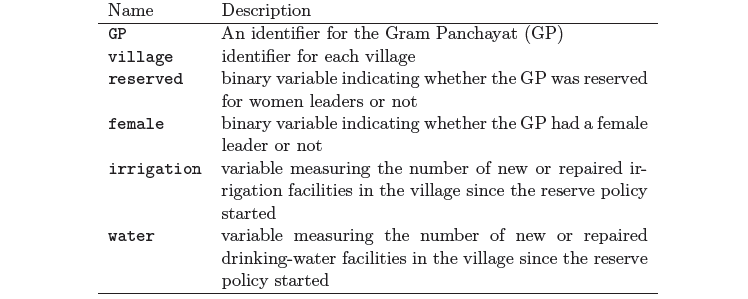
\includegraphics[width=1.1\textwidth]{women_desc.png}
\end{figure}		

\newpage
\begin{enumerate}
	\item [(a)] State a null and alternative (two-tailed) hypothesis. 
	
	H1: 
	In villages where the Gram Panchayat (GP) was reserved for women leaders, the number of new or repaired drinking water facilities differs in a statistically significant manner from the number of new or repaired drinking water facilities in villages where the GP was not reserved for women leaders.
	
	H0:
	In villages where the Gram Panchayat (GP) was reserved for women leaders, the number of new or repaired drinking water facilities does not differ in a statistically significant manner from the number of new or repaired drinking water facilities in villages where the GP was not reserved for women leaders.
	
	\item [(b)] Run a bivariate regression to test this hypothesis in \texttt{R} (include your code!).
	
	Testing the association between water (number of new or repaired drinking-water facilities in the village since the reserve policy started) and reserved (was the GP reserved for women leaders or not) in the dataset.
	\begin{verbatim}	
		> lm(water~reserved, data = women_df)
		
		Call:
		lm(formula = water ~ reserved, data = women_df)
		
		Coefficients:
		(Intercept)     reserved  
		14.738        9.252  
	\end{verbatim}
	
	\item [(c)] Interpret the coefficient estimate for reservation policy. 
	
	This coefficient specifically represents the estimated effect of the reservation policy (Gram Panchayat reserved for women) on the number of new or repaired drinking water facilities in the villages. 
	In this case, it means that villages with the reservation policy are expected to have, on average, 9.252 more new or repaired drinking water facilities compared to villages without the reservation.
	This also means that the reservation policy is associated with an average increase of 9.252 new or repaired drinking water facilities in villages where the GP is reserved for women, compared to those where it is not.
\end{enumerate}

\end{document}
